\newcommand{\polynomial}[4]{% #1 = x position, y_position, #3 = number of squares, label
	\foreach \j in {0,...,\numexpr#3-1\relax} {
		\draw (#1+\j, #2) rectangle (#1+\j+1, #2+1);
	}
	  \node[anchor=center, inner sep=2pt] (#4) at (#1 + #3/2, #2+0.5) {};
}

\newcommand{\coloredPolynomial}[4]{% #1 = x position, y_position, #3 = number of squares, label
	\foreach \j in {0,...,\numexpr#3-1\relax} {
		\draw[fill=blue, opacity=10] (#1+\j, #2) rectangle (#1+\j+1, #2+1);
	}
	\node[anchor=center, inner sep=2pt] (#4) at (#1 + #3/2, #2+0.5) {};
}


	\def\numSquares{5}
\def\spacingPoly{2}


\newcommand{\mvbFigureA}{
	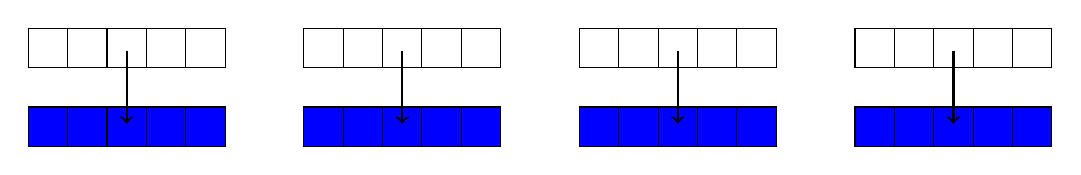
\begin{tikzpicture}[scale=0.5, transform shape]
		\foreach \i in {0,...,3} {
			\pgfmathsetmacro{\xpos}{(\numSquares + \spacingPoly) * \i}
			\polynomial{\xpos}{0}{\numSquares}{poly\i}
			
			\coloredPolynomial{\xpos}{-2}{\numSquares}{polyBis\i}
			
			\draw[->, thick] (poly\i.south) -- (polyBis\i.north);
			
			\node[anchor=west] at (\xpos + \numSquares/2, -0.5) {\BlindRotate};
		}
	
	\end{tikzpicture}
}


\newcommand{\mvbFigureB}{
	\begin{tikzpicture}[scale=0.5, transform shape]
		\pgfmathsetmacro{\xpos}{(\numSquares + \spacingPoly) * 1.5}
		\polynomial{\xpos}{-4}{\numSquares}{polyBeforeMVB}
		
		\coloredPolynomial{\xpos}{-6}{\numSquares}{polyDuringMVB}
		\draw[->, thick] (polyBeforeMVB.south) -- (polyDuringMVB.north);
		\node[anchor=west] at (\xpos+ \numSquares/2 , -4.5) {\BlindRotate};
		
		\foreach \i in {0,...,3} {
			\pgfmathsetmacro{\xpos}{(\numSquares + \spacingPoly) * \i}
			\coloredPolynomial{\xpos}{-9}{\numSquares}{polyAfterMVB\i}
	
			\draw[->, color=purple, thick] ($(polyDuringMVB.south) + (0, -0.5)$) -- (polyAfterMVB\i.north);
			
			\node[anchor=west] at (\xpos + 1, -7.7) {\huge $\times v_\i$};
		}
	\end{tikzpicture}
}
